\documentclass[10pt, a4paper]{amsart}

\usepackage[]{graphicx}
\usepackage{subcaption}
\usepackage[toc,page]{appendix}
\usepackage[]{hyperref}
\usepackage[]{physics}
\usepackage[]{listings}
\usepackage[utf8]{inputenc}
\usepackage[dvipsnames]{xcolor}

\definecolor{mygray}{gray}{0.9}

\lstset{
	frame = single,
	language = C++,
	showstringspaces = false,
	tabsize = 2,
	otherkeywords = {self},
	keywordstyle = \color{Maroon},
	identifierstyle=\color{olive},
 	stringstyle=\color{orange},
 	backgroundcolor=\color{mygray},
 	breaklines = true
}

\title[Simulation of monetary transactions]{Monte Carlo simulation of monetary transactions: \\
\normalsize{A simple model for wealth distribution} \\
  \hrulefill\small{ FYS3150: Computational Physics }\hrulefill}

\author[Svalheim \& Winther-Larsen]{Trygve Leithe Svalheim \\
   Sebastian G. Winther-Larsen \\
  \href{https://github.com/gregwinther/FYS3150/}{\texttt{github.com/gregwinther}}}
  

\begin{document}

\begin{titlepage}
\begin{abstract}
Lorem ipsum dolor sit amet, consectetur adipiscing elit. In id neque elementum, accumsan ligula at, lobortis tortor. Duis elementum pellentesque purus, sit amet euismod diam facilisis volutpat. Nulla facilisi. Mauris quis felis ante. Aliquam ac velit sit amet velit porta condimentum iaculis ut quam. Phasellus pretium libero nec lectus placerat, ac consectetur sem faucibus. Maecenas dictum porta finibus.
\end{abstract}
\maketitle
\tableofcontents
\end{titlepage}

%% -----------------
%% INTRODUCTION
\section{Introduction}


%% -----------------
%% THEORY
\section{Theoretical Background}
\subsection{The simplest model for an economy}
Arguably, the most famous equation in macroeconomics is the ``autarky identity"\footnote{Any introductory text on macroeconomics will give a thorough elaboration, e.g. Gärtner.}
\begin{equation}
\label{eq:YCGI}
Y = C + G + I,
\end{equation}
where $Y$ is income, $C$ is consumption, $G$ is government spending and $I$ is investment. The best-know, but not necessarily the best, measure of income $Y$ is the Gross Domestic Product (GDP)\footnote{GDP = GNP (Gross National Product) in autarky.}. Consumption $C$ is the monetary value of all goods and services purchased in the private sector, while government spending $G$ is the consumption of the government. Finally, investment $I$ is the sum of private and public saving. 

Equation \ref{eq:YCGI} is autarkic because all interactions with other economies are excluded from the expression. There are no terms representing exports and captial inflow, for instance. We are dealing with a \emph{closed} economy, alternatively the entire world as a whole. Moreover, let's assume that the economy we are studying is a peaceful anarchy, without a governing authority of any sort, in effect setting $G = 0$. To begin with, we will also forgo the agents the ability to save such that the worth of every individual, or agent, in the economy must be spent at once. Equation \ref{eq:YCGI} is reduced to $Y = C$, everything one agent spends is the income of another.

\subsection{Monetary transactions}
To simulate monetary transactions in our model economy we expand employ the framework introduced in Patriarca et al.\cite{Patriarca}. We assume there are $N$ agents that exchange money in pairs ($i,j$). We assume also that all agents start with the same amount of money $m_0>0$. For every period an arbitrary pair of agents are picked at randomly and let them conduct business, id est a transaction takes place between them. Money is conserved during the transaction such that
\begin{equation}
\label{eq:wealthconserved}
m_i + m_j = m_i' + m_j',
\end{equation}
where the right-hand side is the agent $i$ and $j$'s updated wealth and the left-hand side represents the amount of money agents $i$ and $j$ had before the transaction. The exchange is done via a random reassignment factor $\epsilon$, such that
\begin{align}
m_i' &= \epsilon (m_i + m_j) \\
m_j' &= (1 - \epsilon) (m_i + m_j)
\end{align}
No agent will ever have negative wealth, that is $m \geq 0$. Moreover, because of the conservation law in equation \ref{eq:wealthconserved}, the system eventually reaches an equilibrium state given by a Gibbs distribution
\begin{equation}
\label{eq:gibbs}
w_m = \beta e^{-\beta m}, \quad \beta = \frac{1}{\ev{m}},
\end{equation}
where $\ev{m}$ is the expected wealth, for which the arithmetic mean is an unbiased estimator. This implies that after an equilibrium has been reached the majority of agents is left with lower wealth than they had initially and
the number of rich agents exponentially decrease.

It is easy to see that the logarithm of the Gibbs measure in equation \ref{eq:gibbs} yields a linear equation
\begin{equation}
\label{eq:lingibbs}
\ln(w_m)=\ln(\beta) - \beta m
\end{equation}

\subsection{Pareto distributions}
How the income and wealth of a population has been studied for a long time. Already in 1897, Vilfredo Pareto, sought to describe bot wealth and income distribution by power law probability distributions\cite{Pareto}. Pareto showed that the higher end of the distribution of money follows a distribution
\begin{equation}
\label{eq:paretodist}
w_m \propto m^{-1-\alpha}, \quad \alpha \in [1,2].
\end{equation}
Pareto's ``80-20 rule", that $20\%$ of the population controls $80\%$ of the wealth, corresponds to a certain value of $\alpha$. Today, a whole class of distributions similar to the one in equation \ref{eq:paretodist} are named after Pareto\cite{Arnold}.

\subsection{Transactions and savings}
We are can expand upon the model by introducing a savings rate $\lambda$. The savings rate is defined as a fraction of an agent's wealth that does not partake in a transaction for every period. One can gather from the macroeconomic identity in equation \ref{eq:YCGI} that income must still be the same and the transaction law in equation \ref{eq:wealthconserved} still holds. The updated wealth of agents $i$ and $j$ after a transaction becomes
\begin{align}
m_i' &= \lambda m_i + \epsilon (1 - \lambda) (m_i + m_j) \\
m_j' &= \lambda m_j + (1- \epsilon) (1 - \lambda) (m_i + m_j)
\end{align}
one can rewrite these expressions to
\begin{align*}
m_i' &= m_i + \delta m \\
m_j' &= m_j - \delta m
\end{align*}
where
\begin{equation}
\delta m = (1 - \lambda)(\epsilon m_j - (1 - \epsilon)m_i)
\end{equation}

\subsection{Economic inequality and social friction}
``The first historical series of income distribution statistics became available with the publication in 1953 fo Kuznet's monumental Shares of Upper Income Groups in Income and Savings. Kuznet's series dealt with only one country (the United Stetes) over a period of thirty-five years (1913-1948)" (Pikkety \& Ganser, 2014, Kindle locations 276-280\cite{Piketty}). Ever since that time there has been wealth and income inequality to a greater or lesser degree. According to the PolitiFact the top 400 richest Americans in 2011 "[had] more wealth than half of all Americans combined"\cite{Moore}.

One of the possible reasons for continued wealth and income inequality that has risen in popularity the last few years is the process of wealth concentration. This is a process by which, under certain conditions, newly created wealth concentrates in the possession of already-wealthy individuals or entities. Those who already have wealth have the means to invest in newly created sources and structures of wealth. Piketty argues that the fundamental force for wealth divergence is the usually greater return of capital than economic growth (Piketty \& Ganser, 2014 p. 284 Table 12.2\cite{Piketty}).

To incorporate the social rigidities described above, we will make two further additions to the model. These additions build mostly on the work of Goswami and Sen\cite{GoswamiSen}. Firstly, we will make it more likely for two agents to conduct a transaction if they have similar wealth. Second, we will make it more likely for two agents to make a transaction if they have made a transaction before. We define a probability
\begin{equation}
\label{eq:rigidprob}
p_{ij} \propto \abs{m_i - m_j}^{-\alpha}(c_{ij}+1)^{\gamma},
\end{equation}
where the first factor $\abs{m_i-m_j}^{-\alpha}$ relates to wealth similarity and the second factor $(c_{ij}+1)^{\gamma}$ relates to previous transactions. A relatively large difference between $m_i$ and $m_j$ should translate to a lower probability. The strength of this effect is governed by the exponent $\alpha$, a larger value decreases the probability of a trade further. The variable $c_{ij}$ is simply the number of times agent $i$ and $j$ have conducted transactions in the past. The number $1$ is added in order to ensure that if they have not interacted earlier they can still interact. The strength of this effect is governed by the exponent $\gamma$.


%% -----------------
%% ALGORITHM
\section{Algorithm \& Implementation}
All programming code used in this project is written in C++ and is publicly available at github by following the link on the first page. The program consists mainly of two files, \lstinline|main.cpp| and \lstinline|functions.cpp|. \lstinline|main.cpp| contains the set-up of the program and is where the number of agents, initial wealth, number of transactions, number of simulations and all parameters ($\lambda$, $\alpha$ and $\gamma$) are specified. The main part of the program however, is in \lstinline|functions.cpp| which in addition to the \lstinline|trade(...)|\footnote{The functions have several arguments: \lstinline|trade(int N, int no_of_transactions, arma::vec (&agents), double lambda, double alpha, double gamma)|. To include all the arguments in the text would have decreased readability and they are replaced with dots.} function contains the function \lstinline|output(...)|\footnote{\lstinline|output(...)| = \lstinline|output(int N, arma::vec agents, std::string filename)|.} which writes data to file.

\subsection{The \lstinline|trade(...)| function}
This function runs a specified number of Monte Carlo cycles, where the transactions take place. For each iteration two random agents are picked, then some logic follows which will determine if the two agents are allowed to go into business. This is a very important part of the program and is therefore listed here:
\begin{lstlisting}
while ((pow(fabs(m_i - m_j), -alpha)*
		pow(previous_transactions+1, gamma) < random_number)
		|| (agent_i == agent_j)) {
      
	// Pick new agents ...
	agent_i = (int) rand() % N;
	agent_j = (int) rand() % N;

	// ... find wealth of these ...
	m_i = agents(agent_i);
	m_j = agents(agent_j);

	// ... update previous transactions ...
	previous_transactions = C(agent_i, agent_j);

	// ... and update the random comparison number
	random_number = (double) rand() / RAND_MAX;
\end{lstlisting}
One can see that the the argument of the while loop in the program listing above contains equation \ref{eq:rigidprob} which is compared against a random number and an equality test that will return \lstinline|True| if agents $i$ and $j$ are the same agent. This part of the code makes sure that a new pair of randomly picked agents until we are satisfied that the agents are not the same and that they are close enough in wealth and in previous relations to go forward with a transaction. After everything is all-right and we have a good pair of agents a transaction takes place:
\begin{lstlisting}
// Random value of transaction b/w 0 and 1
double epsilon = (double) rand() / RAND_MAX;

// Transaction takes place, but some is saved (lambda)
double delta_m = (1 - lambda) * 
	(epsilon*m_j - (1 - epsilon)*m_i);
agents(agent_i) += delta_m;
agents(agent_j) -= delta_m;

// Register that a transaction has taken place
C(agent_i, agent_j) += 1;
C(agent_j, agent_i) += 1;
\end{lstlisting}
The program listing above should be straight-forward. Notice that the transaction is registered in matrix \lstinline|C| by incrementing element $i,j$ and $j,i$ by $1$.

The last part of the \lstinline|trade(...)| function is not particularly important for the quality of the data that a simulation will provide, but vastly increased the speed of the program. This last functionality breaks the for loop within the \lstinline|trade(...)| function when a steady state is reached. Listed in its entirety here:
\begin{lstlisting}
double var = arma::var(agents);
cumVarBlock += var;
cumVar2Block += var*var;

// Enter here at the correct place: end of block
if (i % blockSize == 0) {
	// Variance of a block "averaged" over the block
	double avgVar  =  cumVarBlock / blockSize;
	double avgVar2 = cumVar2Block / blockSize;

	// Variance of a block of variance
	double varVarBlock = avgVar2 - avgVar*avgVar;

	// Check if variance is low enough
	if ((fabs(avgVarBlockOld - avgVar) / fabs(avgVarBlockOld)     < 0.2) &&
		(fabs(varVarBlock - varVarBlockOld) / fabs(varVarBlockOld) < 0.5)) {

		// Telling a user that an equilibrium has been reached
		std::cout << "Equilibrium reached at transaction no. " << i << std::endl;

		// Done! For now.
		break;

		} else {
			avgVarBlockOld = avgVar;
			varVarBlockOld = varVarBlock;
		}
	// Reset cumulative variance
	cumVarBlock  = 0;
	cumVar2Block = 0;
}
\end{lstlisting}
This code section does some calculations on the results after a certain amount of transactions have taken place, an amount predetermined by \lstinline|blockSize|. The average variance of the block is computed as well as the average square variance of the block size. Then the "variance of the variance" is computed. These measures are compared against the measures from the previous block. The relative size of the average variance must be less than $20\%$ and the relative size of the variance of the variance must be less than $50\%$ of the measures from the previous block. If both these logical statements evaluate to \lstinline|True|, the for loop of the \lstinline|trade(...)| function is broken, terminating the current simulation. We found that for most simulations an equilibrium is reached quite quickly, usually between $40000$ and $120000$ transactions have taken place between $N=1000$ agents. This speeds up the time for a simulation to finish tremendously, compared with the initially, and rather naively, picked $10^7$ iterations. In order to find correct values \lstinline|blockSize| as well as when the variance measures are ``low enough'' the behaviour of the variance measures were meticulously studied through several trial runs of the function.

\subsection{Example \lstinline|main()|}
The parameters of the simulation is set up in the \lstinline|main()| function. When all parameters are chosen the following for loop is almost everything that is needed
\begin{lstlisting}
// Start simulations
for (int i = 0; i < simulations; i++) {

	// Print progress
	std::cout << "Simulation no. " << i << std::endl;

	// Assign intitial wealth to all agents
	agents.fill(m0);

	// Trade!
	trade(N, transactions, agents, lambda, alpha, gamma);

	// Sort and add equilibrium wealth to total
	totagents += arma::sort(agents);
\end{lstlisting}
One can see that what must be specified is the number of simulations (\lstinline|simulations|), initial wealth (\lstinline|m0|), number of agents (\lstinline|N|), number of transactions (\lstinline|transactions|), an array containing the wealth of every agent (\lstinline|agents|), savings rate (\lstinline|lambda|), parameter governing weight of wealth similarity (\lstinline|alpha|) and parameter governing weight of past transactions (\lstinline|gamma|).


%% -----------------
%% RESULTS
\section{Results}

%% Problem a, b, c.

Figure \ref{fig:distribution} shows plot of different wealth distributions after $1000$ simulations for $N=500$ agents. We see that that without savings, the distribution shows a decreasing number of agents as wealth increases. As the savings rate $\lambda$ is allowed to increase, the distribution moves to the right and eventually peaks at the initial wealth $m_0 = 100$ when $\lambda = 0.9$. This plot, were it not for the colors, could be an exact copy of figure 1 in Patriarca et al.\cite{Patriarca}. Without savings the distribution appears as a inverse exponential function ($e^{-x}$) which is the same class of function as the Gibbs distribution (equation \ref{eq:gibbs}). However, these traits disappear from the wealth distributions once savings are allowed.

A further study of the wealth distributions from figure \ref{fig:distribution} is visualized in figure \ref{fig:logplot}. Figure  \ref{fig:logdistribution} shows the same graphs as in figure \ref{fig:distribution}, but on with logarithmic scales on both axes. Figure \ref{fig:straightline} the wealth values evaluated by equation \ref{eq:gibbs} and plotted with logarithmic $y$-axis. Observe that all all the wealth distributions give straight lines. This makes sense, as the logarithm of the Gibbs distribution yields a first order expression (equation \ref{eq:lingibbs}).

Figure \ref{fig:paramfig1} shows two different Pareto distributions with $\alpha=1.8$ and $\alpha = 2$ (equation \ref{eq:paretodist}) plotted against a distribution at $\lambda = 0$. We see that they fit adequately with the higher end of the distribution, but not perfectly. The simple Pareto distribution becomes a straight line because of the logarithmic axes in the plot. The same figure also contains a parametrization of the wealth \footnote{This is done in the way Partriarca et al. (2004)\cite{Patriarca} does. A recipe is shown in appendix \ref{app:partriarca}}. Figure \ref{fig:paramfig2} also shows such a parametrization, but for a higher savings rate $\lambda=0.9$. The parametrisations are indicated by a label $P(x)$.


\begin{figure}
	\centering
	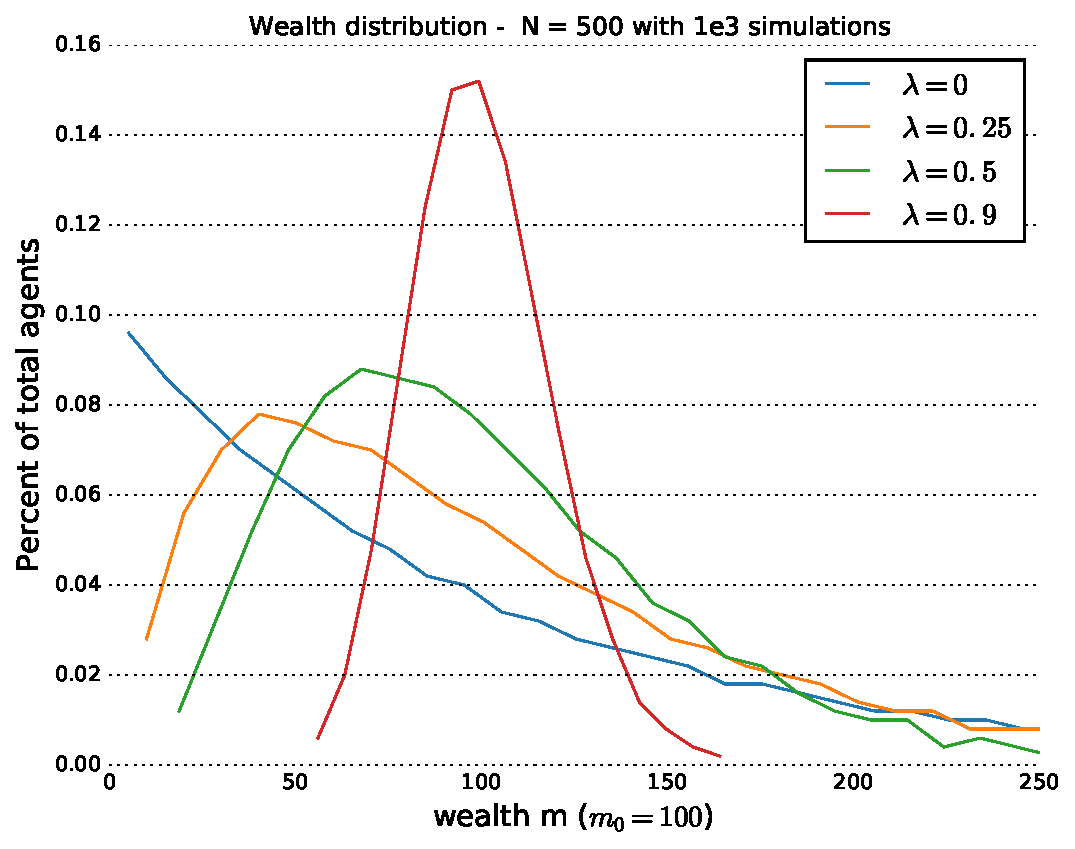
\includegraphics[width=0.9\textwidth]{../figures/5ac/5c_N500_varSavings.pdf}
	\caption{Wealth distribution for $N=500$ agents after $1000$ simulations at different savings rates $\lambda$}
	\label{fig:distribution}
\end{figure}

\begin{figure}
\begin{subfigure}{.5\textwidth}
  \centering
  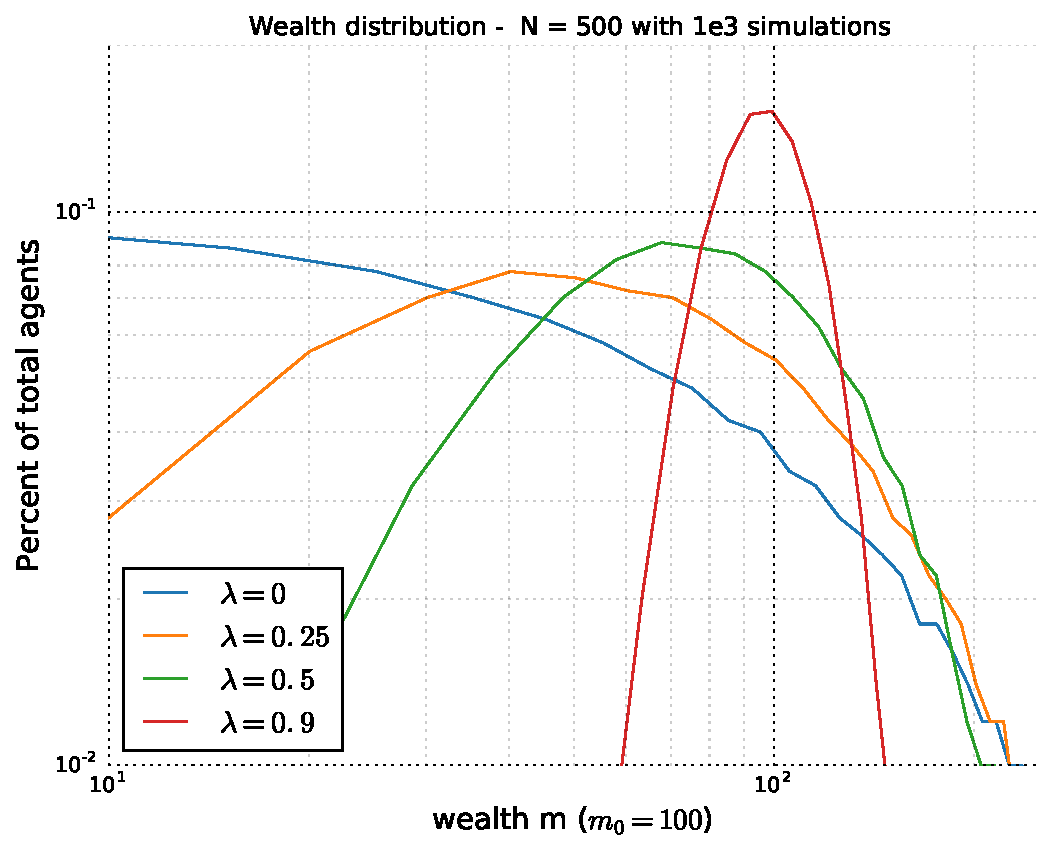
\includegraphics[width=\textwidth]{../figures/5ac/5cLOGLOG_N500_varSavings.pdf}
  \caption{}
  \label{fig:logdistribution}
\end{subfigure}%
\begin{subfigure}{.5\textwidth}
  \centering
  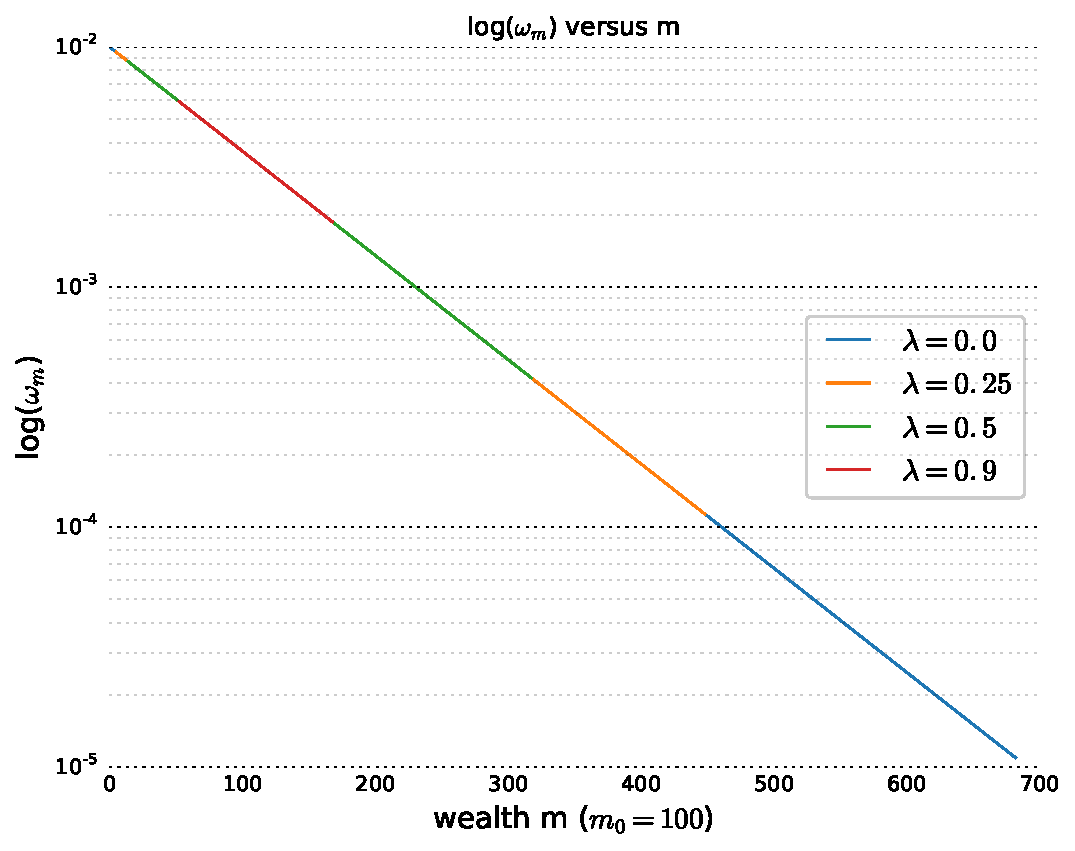
\includegraphics[width=\linewidth]{../figures/5ac/omega.pdf}
  \caption{}
  \label{fig:straightline}
\end{subfigure}
\caption{Logarithmic plot wealth distribution from figure \ref{fig:distribution} (right), and the logarithm of the Gibbs measure (equation \ref{eq:gibbs}) of every data point (right).}
\label{fig:logplot}
\end{figure}

\begin{figure}
\begin{subfigure}{.5\textwidth}
  \centering
  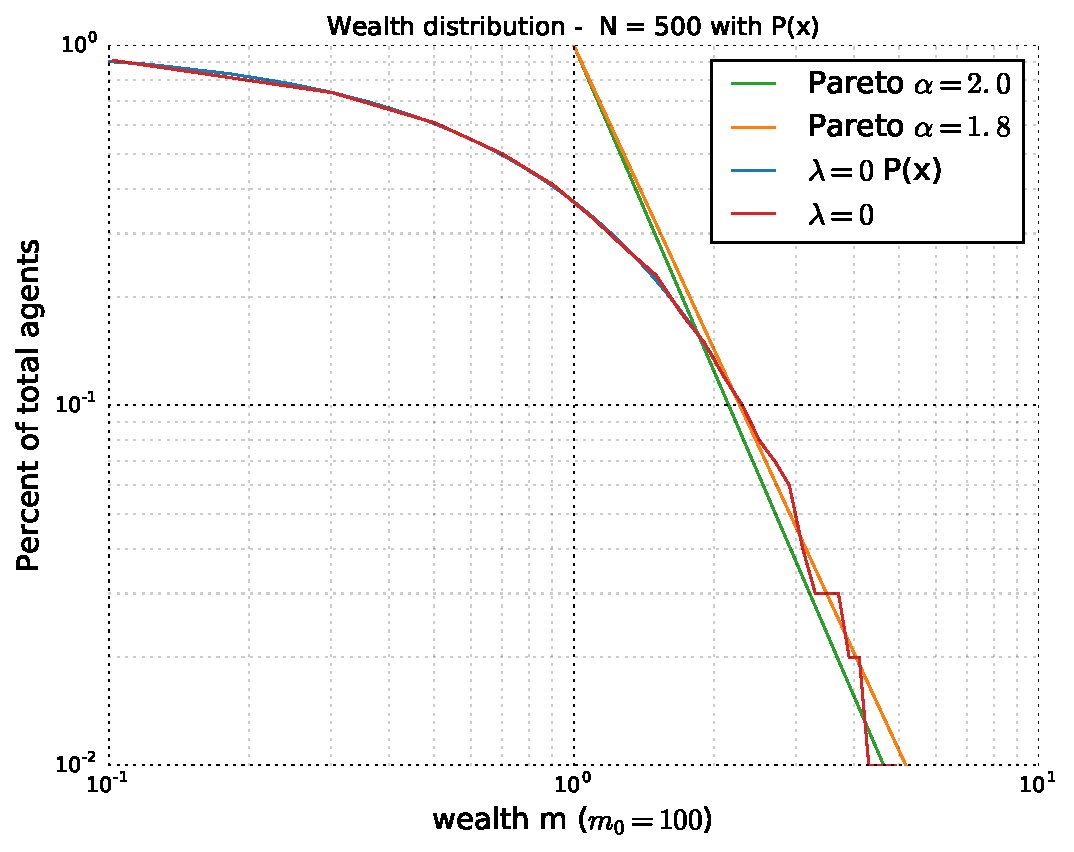
\includegraphics[width=\linewidth]{../figures/5ac/5c_parameterization0.pdf}
  \caption{}
  \label{fig:paramfig1}
\end{subfigure}%
\begin{subfigure}{.5\textwidth}
  \centering
  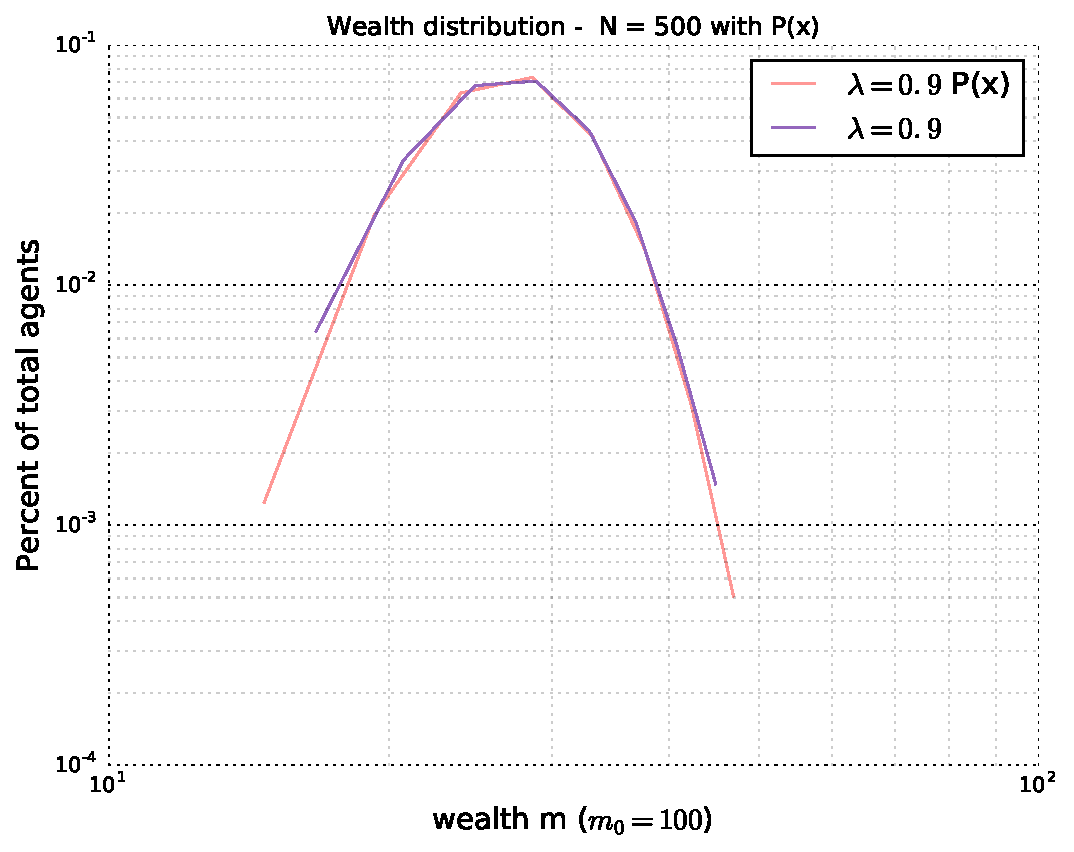
\includegraphics[width=\linewidth]{../figures/5ac/5c_parameterization09.pdf}
  \caption{}
  \label{fig:paramfig2}
\end{subfigure}
\caption{Parametrization of two different wealth distributions, $\lambda=0$ and $\lambda=0.9$. Method for parametrization is found in appendix \ref{app:partriarca}. For $\lambda=0$ two Pareto power law distributions are also shown.}
\label{fig:paramfig}
\end{figure}

%% Problem d.
\begin{figure}
\begin{subfigure}{.49\textwidth}
	\centering
	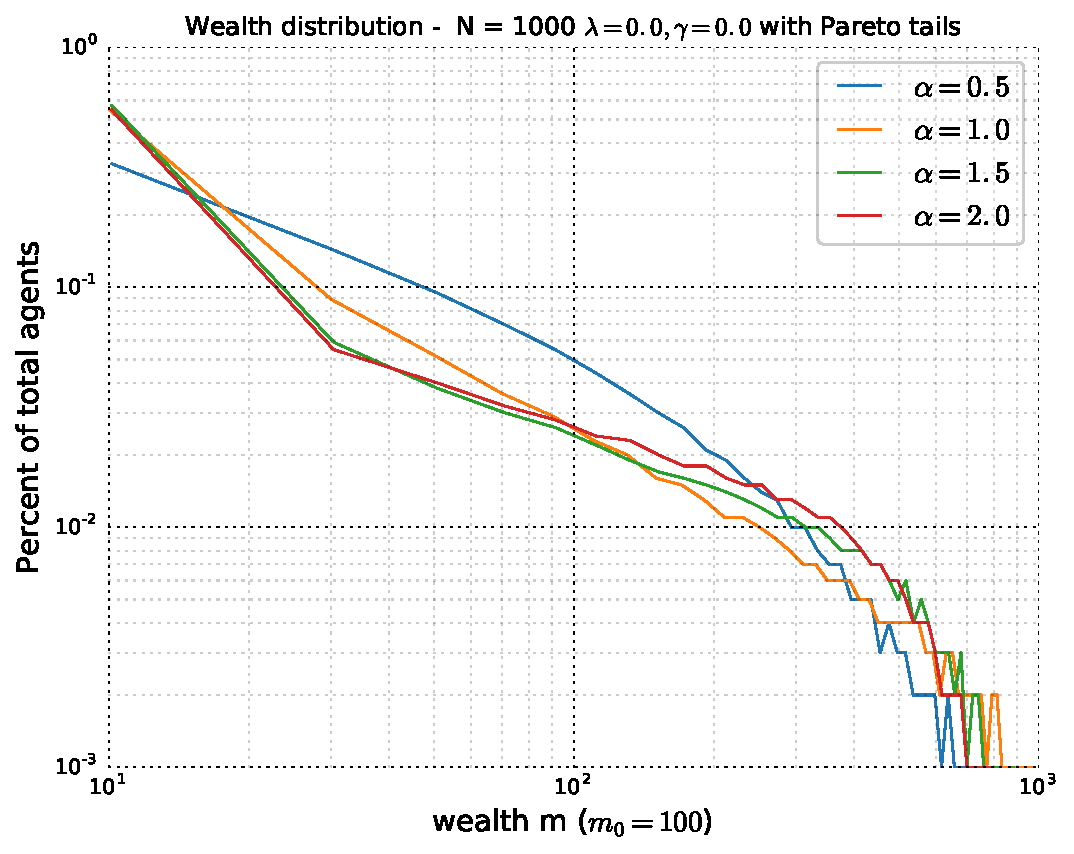
\includegraphics[width=\linewidth]{../figures/5d/5d_0-var-0.pdf}
	\caption{}
	\label{fig:neighbour1}
\end{subfigure}
\begin{subfigure}{.49\textwidth}
	\centering
	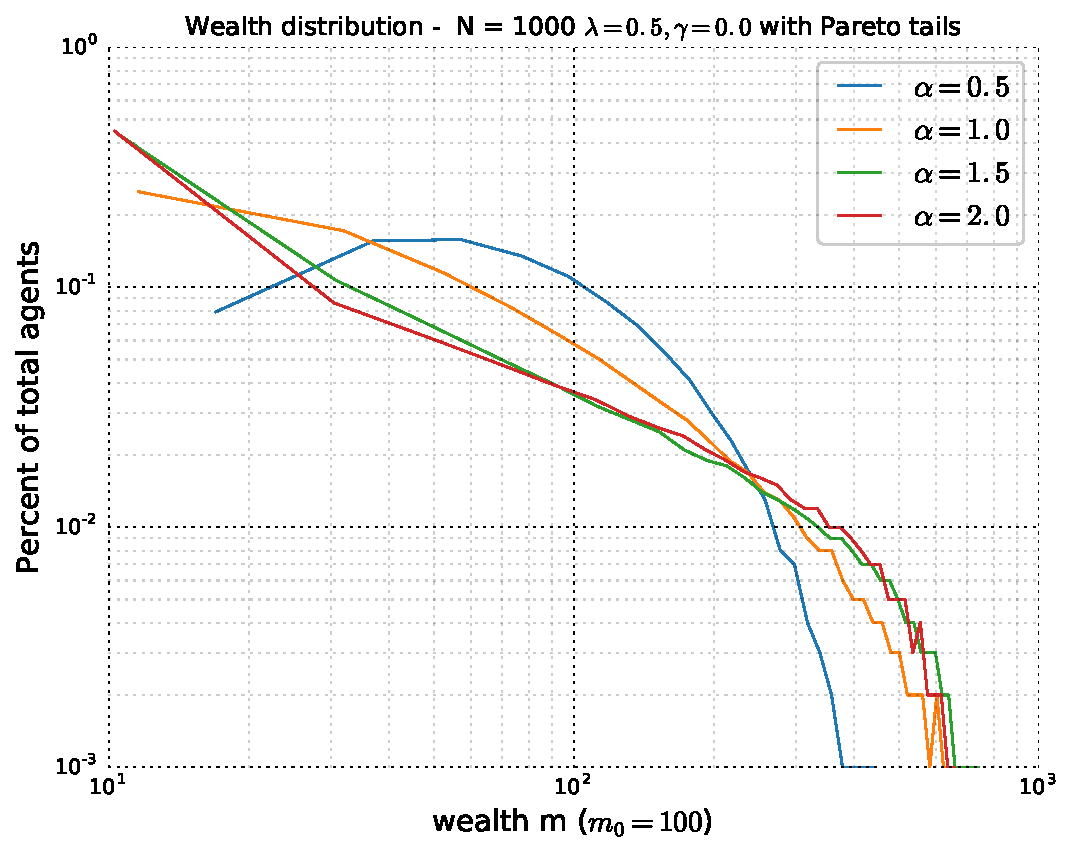
\includegraphics[width=\linewidth]{../figures/5d/5d_05-var-0.pdf}
	\caption{}
	\label{fig:neighbour2}
\end{subfigure}
\caption{Effect of neighbour-only interaction}
\end{figure}

\begin{figure}
\begin{subfigure}{.49\textwidth}
	\centering
	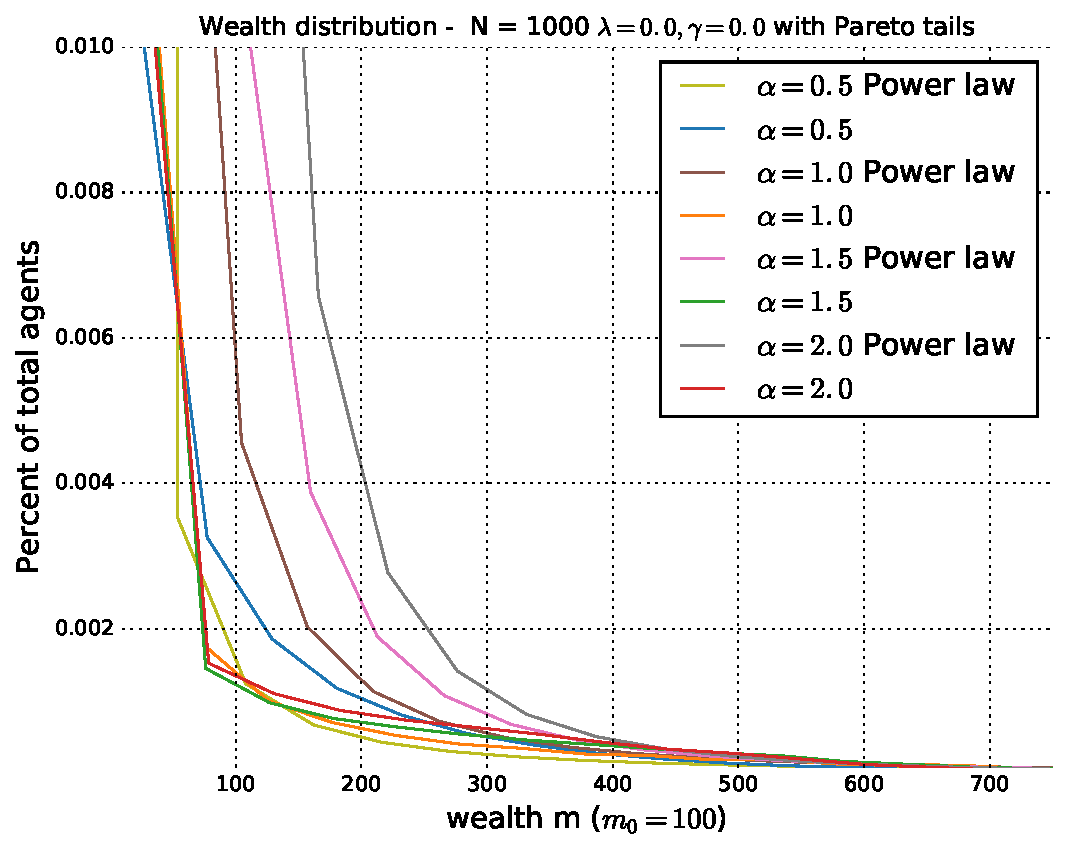
\includegraphics[width=\linewidth]{../figures/5d/5d_0-var-0-PARETO.pdf}
	\caption{}
	\label{fig:neighbourpareto1}
\end{subfigure}
\begin{subfigure}{.49\textwidth}
	\centering
	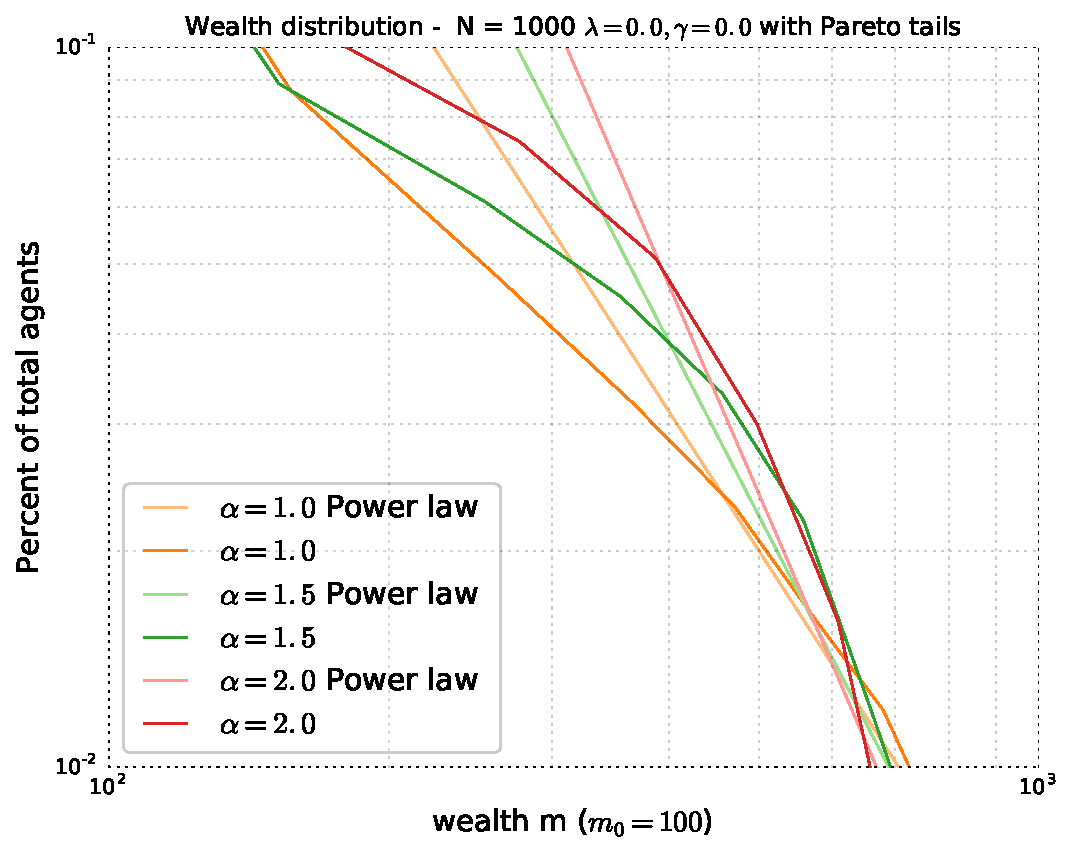
\includegraphics[width=\linewidth]{../figures/5d/5d_0-var-0-POWERLOG.pdf}
	\caption{}
	\label{fig:neighourpareto2}
\end{subfigure}
\caption{Effect of neighbour-only interaction}
\end{figure}


%% ----------------
%% DISCUSSION
\section{Discussion}

%% ---------------
%% CONCLUSION
\section{Summary Remarks}


\begin{thebibliography}{10}

\bibitem{Patriarca} Patriarca, M., Chakraborti, A., \& Kaski, K. (2004). 
	Gibbs versus non-Gibbs distributions in money dynamics. 
	\emph{Physica A: Statistical Mechanics and its Applications},
	340(1), 334-339.
	
\bibitem{Pareto} Pareto, V. (1897).
	\emph{Cours d'Économique politique},
	Lausanne: Ed. Rouge.

\bibitem{Arnold} Arnold, B. C. (1983). 
	\emph{Pareto Distributions}.
	 International Co-operative Publishing House	

\bibitem{Piketty} Piketty, T., \& Goldhammer, A. (2014).
	\emph{Capital in the twenty-first century},
	Cambridge: Harvard University Press.
	
\bibitem{Moore} Moore, M., (March 7, 2011).
	The Forbes 400 vs. everybody else.
	\emph{\href{https://web.archive.org/web/20110309211959/http://www.michaelmoore.com/words/must-read/forbes-400-vs-everybody-else}{michaelmoore.com}}.
	Retrieved December 8. 2016.

\bibitem{GoswamiSen} Goswami, S., \& Sen, P. (2014).
	Agent based models for wealth distribution with preference in interaction.
	\emph{Physica A: Statistical Mechanics and its Applications},
	415, 514-524.

\end{thebibliography}

\begin{appendices}

\section{Parametrization from Patriarcal et al.}
\label{app:partriarca}
A corresponding exact solution of an income distributions for a generic value of $\lambda$ with $0<\lambda<1$ is provided in Patriarca et al.\cite{Patriarca}. Fir one employs the reduced variable
\begin{equation}
x = \frac{m}{\ev{m}}
\end{equation}
the agent money in units of average money $\ev{m}$ and the parameter
\begin{equation}
n(\lambda) = 1 + \frac{3\lambda}{1-\lambda}.
\end{equation}
The money distributions, for arbitrary values of $\lambda$, are well fitted by the function
\begin{equation}
P_n(x) = a_nx^{n-1}e^{-nx}
\end{equation}
where $a_n$ is a normalization factor shown to be
\begin{equation}
a_n = \frac{n^n}{\Gamma(n)}
\end{equation}
\end{appendices}

\end{document}
